% !TEX root = manuscript.tex

\chapter{Nettoyage, Exploration et Analyse descriptive des données}
\minitoc
\newpage
\section{Nettoyage et Analyse du jeu de données train}


\subsection{Statistique descriptive des données train }
Le jeu de donnée d'entrainement (train), dispose de 7500 lignes et 18 colonnes. L'analyse descriptive (voir figure \ref{fig:stat_descriptive}) de ce dernier nous montre que les colonnes Annual Income, Months since last delinquent, Credit Score et Years in current qui contiennent plusieurs valeurs manquantes(Na). Par la suite, nous avons utilisé la médiane pour la gestion des valeurs manquantes. 

\begin{figure}[H]
\centering
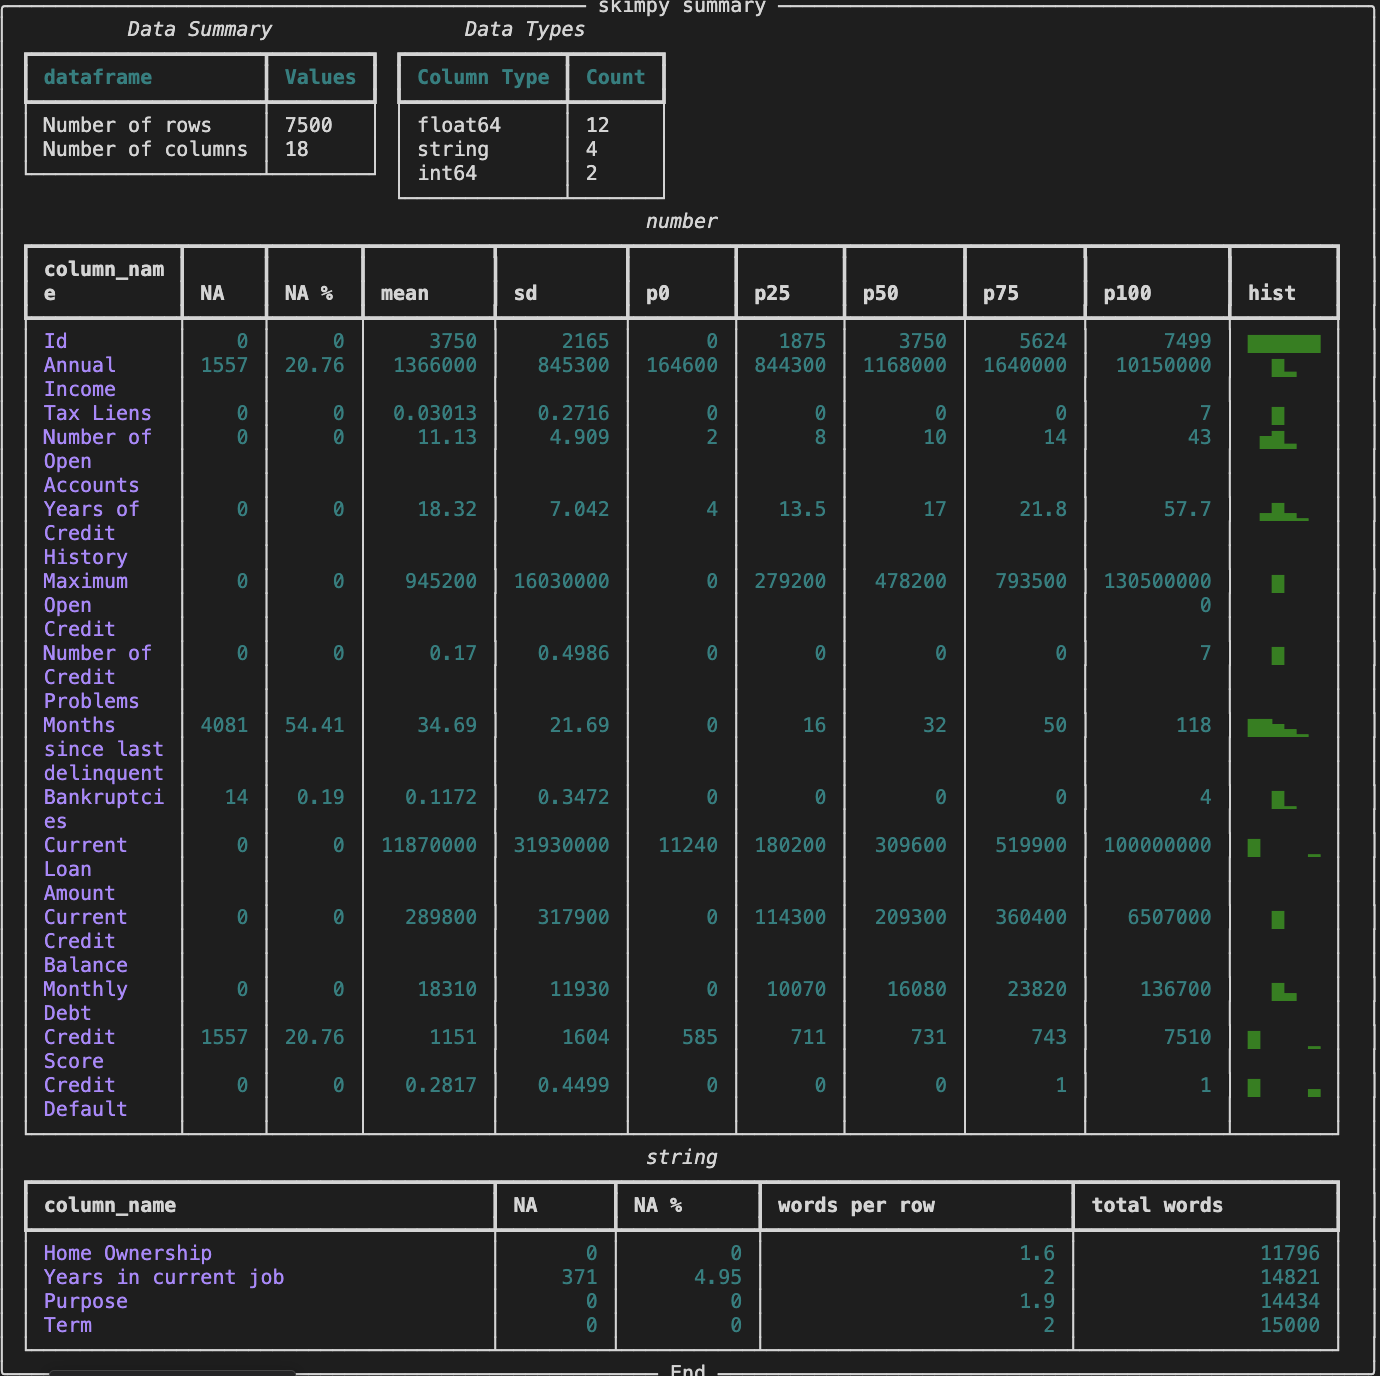
\includegraphics[width=0.8\textwidth]{figures/fig1.png}
\caption{Statistique descriptive train.}
\label{fig:stat_descriptive}
\end{figure}

\subsection{Matrice de corrélation}
\begin{flushleft}
\begin{enumerate}
\item Nous allons dans un premier temps représenter la matrice de corrélation avec les colonnes numériques(voir figure \ref{fig:matrice_corr}). 
\begin{flushleft}
On note une très faible correlation linéaire entre le Credit Default et les autre variables quantitative.

De même, on note d'une part une faible liaison négative entre Credit Default et Current Loan Amont et d'autre part une faible liaison postive entre Credit Default et Credit Score

Certaines colonnes ont des corrélations très faibles (proches de 0), ce qui peut indiquer qu'elles n'ont pas d'impact direct sur Credit Default.
\end{flushleft} 

\begin{figure}[H]
\centering
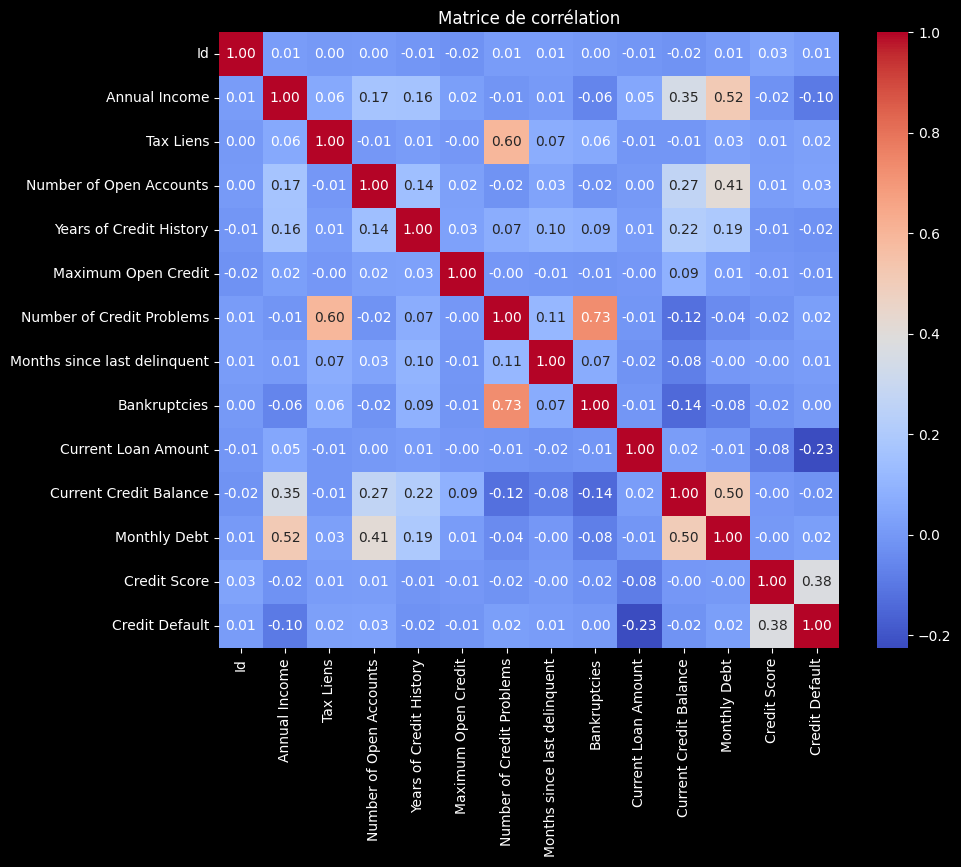
\includegraphics[width=0.8\textwidth]{figures/Matrice1.png}
\caption{Matrice de corrélation.}
\label{fig:matrice_corr}
\end{figure}


\item Par la suite, nous avons utilisé la technique d'encodage \textbf{LabelEncoder} pour encoder la colonne \textbf{Years in current job}, puis avons utilisé \textbf{One-Hot Encoding} pour encoder les autres colonnes catégorielles. 
\end{enumerate}
\end{flushleft}
\begin{flushleft}

La corrélation la plus élevée avec Credit Default est pour Credit Score (0.44), ce qui peut indiquer une relation modérée entre ces deux variables.
Term\_Long Term et Term\_Short Term ont des corrélations opposées (0.181 et -0.181), ce qui est logique car elles sont mutuellement exclusives dans un encodage one-hot.

Certaines colonnes ont des corrélations très faibles (proches de 0), ce qui peut indiquer qu'elles n'ont pas d'impact direct sur Credit Default.


Pour soumettre notre jeu de données train aux différents modèles de classification, nous avons besoin de convertir nos colonnes issues du \textbf{pd.get\_dummies()} en de type \textbf{int}, cela facilitera leur traitement dans certains modèles ou calculs. Par la suite nous allons normaliser les colonnes pour éviter les biais dus à des échelles différentes. (Voir le résumé statistique après analyse et traitement des données à l'annexe Annexe~\ref{sec:annexe3}).
\end{flushleft}

\section{Nettoyage et Analyse du Jeu de donnée test}
\subsection{Statistiques descriptives}

Le jeu de donnée d'entrainement (train), dispose de 2500 lignes et 17 colonnes. L'analyse descriptive (voir figure \ref{fig:stats_descriptive}) de ce dernier nous montre que les colonnes Annual Income, Months since last delinquent, Credit Score et Years in current qui contiennent plusieurs valeurs manquantes(Na). Par la suite, nous avons utilisé la médiane pour la gestion des valeurs manquantes. (voir Annexe~\ref{sec:annexe4}).

\begin{figure}[H]
\centering
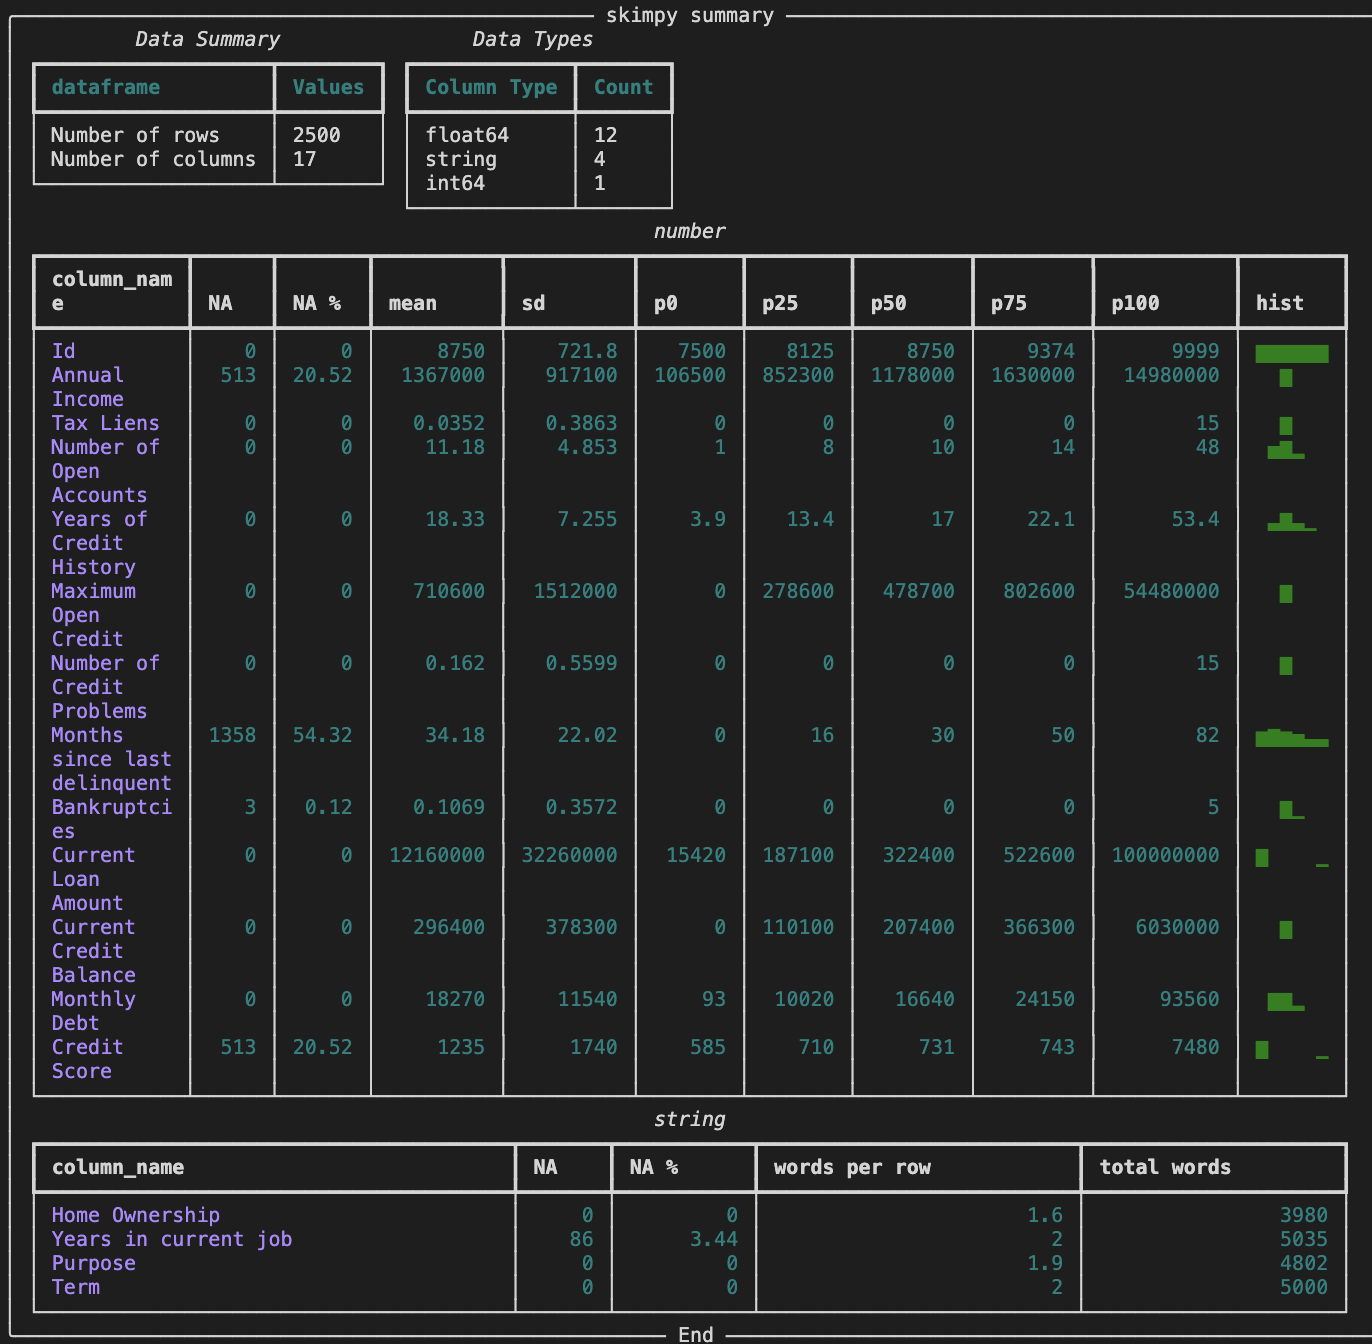
\includegraphics[width=0.8\textwidth]{figures/fig2.png}
\caption{Statistique descriptive test.}
\label{fig:stats_descriptive}
\end{figure}


\subsection{Traitement du jeu de donnée test}

Nous avons utilisé les mêmes techniques de nettoyage, de normalisation, de standardisation et d'encodage sur le jeu de donnée test. (voir le résumé statistique après nettoyage à l'annexe Annexe~\ref{sec:annexe4}). 

